\documentclass[oneside,a4paper,10pt]{article}
\usepackage[english,brazilian]{babel}
\usepackage[alf]{abntex2cite}
\usepackage[utf8]{inputenc}
\usepackage[T1]{fontenc}
\usepackage[top=5mm, bottom=5mm, left=5mm, right=5mm]{geometry}
\usepackage{framed}
\usepackage{booktabs}
\usepackage{color}
\usepackage{hyperref}
\usepackage{graphicx}
\usepackage{float}
\graphicspath{{./Figuras/}}    
\usepackage{multicol}
\definecolor{shadecolor}{rgb}{0.8,0.8,0.8}

\newcommand{\EREM}{EREM Regina Pacis}
\newcommand{\curso}{\textbf{3 EMSI}}
\newcommand{\professor}{Prof. Leandro Vieira}

\begin{document}
\pagestyle{empty}
análise de gráficos

\begin{center}
\EREM
\par %pula uma linha
\curso
\par
\professor
\par
\LARGE \textbf{Atividade de Matemática}
\end{center}

\begin{enumerate}

\item Para melhorar a organização e prestação de contas de uma lanchonete, o gerente organizou os dados da receita média diária no gráfico a seguir:

\begin{figure}[h]
\center
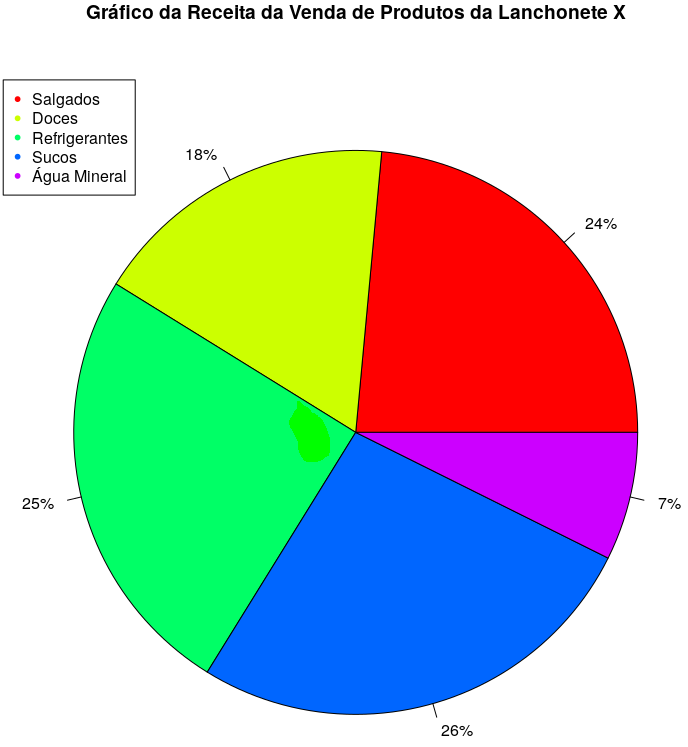
\includegraphics[width=8cm]{Figuras/g1.png}
\end{figure}

Sabendo que a receita da venda de salgados dessa lanchonete foi de R\$550,00. Responda os ítens a seguir:
	\begin{enumerate}
	\item Qual o percentual de vendas de salgados dessa lanchonete:
	\item Qual o total da receita obtida por essa lanchonete diariamente:\
	\item Qual a receita de vendas de doces:
	\item Sabendo que a lanchonete ficou aberta durante 25 dias do mês. Calcule qual foi o seu lucro no mês na venda de refrigerantes, uma vez que a porcentagem de lucro nesse produto é de 25\%:
	\end{enumerate}


\end{enumerate}

\flushbottom 
\flushright
"A arte de viver é simplesmente a arte de conviver...\\Simplesmente, disse eu? Mas como é difícil!\\(Mario Quintana)

\end{document}